\section{S4 -- Technologie platformy Java EE}

Java Platform, Enterprise Edition znana jako Java EE (nie używać JEE \url{https://java.net/projects/javaee-spec/pages/JEE}) to \textbf{specyfikacja} platformy programistycznej Java. Nie jest to implementacja, a tak naprawdę rozszerzenie wersji SE o komponenty (interfejsy) sieciowe, które umożliwiają pisanie aplikacji o przeznaczeniu komercyjnym. Twórcą tej technologi był \textit{Sun Microsystems}, ale kupił go \textit{Oracle}. 
DO uruchomienia aplikacji potrzebny jest serwer aplikacji Java EE. Do najczęściej używanych i zarazem najpopularniejszych serwerów należą:
\begin{itemize}
    \item Apache Tomcat
    \item GlassFish
    \item IBM WebSphere
    \item JBoss Application Server
\end{itemize}

\textbf{Cechy Java EE}
\begin{itemize}
    \item bezpieczeństwo,
    \item skalowalność,
    \item przenośność,
    \item wielowarstwowość.
\end{itemize}

Aplikację napisaną zgodnie ze standardem Java EE można podzielić na minimum 3 warstwy:

\begin{figure}[H]
\centering
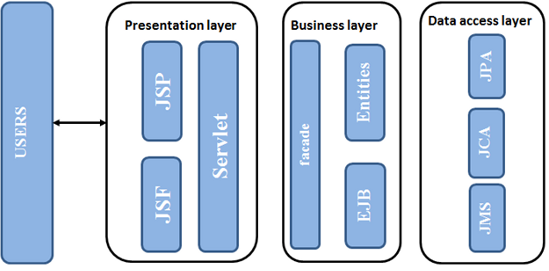
\includegraphics[width=\linewidth]{s4_int_warstwy.png}
\caption{Warstwy aplikacji Java EE}
\end{figure}

\begin{itemize}
    \item Warstwa prezentacji -- w tej warstwie zdefiniowany jest interfejs użytkownika.
    \item Warstwa biznesowa -- tworzenie komponentów implementujących logikę biznesową.
    \item Warstwa dostępu do danych -- zapewnia izolację danych. 
\end{itemize}

W warstwie prezentacji można wyróżnić 3 zasadnicze sposoby generowania interfejsu użytkownika.

\textbf{JSF} --  framework, bazujący na języku Java, który upraszcza tworzenie interfejsu użytkownika do aplikacji Java EE. Obecnie domyślną technologią widoku dla stron JSF jest technologia Facelets. Składa się z kontrolek umożliwiających szybkie tworzenie interfejsu użytkownika.

\textbf{JSP} --  to technologia umożliwiająca tworzenie dynamicznych dokumentów WWW w formatach HTML, XHTML, DHTML oraz XML z wykorzystaniem języka Java, wplecionego w kod HTML danej strony. W tym aspekcie, jest to rozwiązanie podobne do PHP. Strona JSP w procesie translacji jest zamieniana na serwlet. Każde wywołanie strony JSP z poziomu klienta (przeglądarki) wykonywane jest przez skompilowany serwlet. 

W części dynamicznej JSP można wykorzystać 5 elementów:
\begin{itemize}
    \item <\%@ dyrektywa \%> 
    \item <\%! deklaracja \%>
    \item <\%= wyrażenie \%>
    \item <\% kod \%>
    \item <\%-- komentarz --\%>
\end{itemize}

Dodatkowo, dzięki użyciu \textbf{JSTL} dodane zostają dodatkowe tagi do \textbf{JSP}, co umożlwia m.in. tworzenie pętli. Tagi te posiadają swoje prefiksy np. Core tags,–c; XML–x; HTML-h. Przykład: <c:forEach...>.

\textbf{Serwlety} -- jest to samodzielna klasa Javy, która dziedziczy po HttpServlet. Zawiera metody niezbędne do obsłużenia zapytania http. Osadzana jest w kontenerze webowym (aplikacja), który wywołuje jej metodę doPost() lub doGet() w celu obsłużenia przychodzącego żądania. Servlet taki wówczas może odesłać odpowiedź, lub przekierować żądanie do innej części aplikacji (sendRedirect). Każde zapytanie realizowane jest w oddzielnym wątku.

Typowe zastosowania serwletu:
\begin{itemize}
    \item przekierowanie do strony JSP,
    \item kontakt z bazą danych,
    \item uwierzytelnianie użytkowników,
    \item sterowanie aplikacją.
\end{itemize}

Cykl życia serwletu składa się z następujących kroków:
\begin{enumerate}
    \item Załadowanie klasy serwletu do pamięci (tylko raz, podczas pierwszego ładowania strony).
    \item Wywołanie konstruktora oraz init().
    \item Instancja rezyduje w pamięci w oczekiwaniu na zapytania. Jeśli nadejdzie nowe zapytanie, serwer tworzy nowe obiekty (request i response) oraz wywołuje service() przekazując request i response do odpowiedniej metody zaimplementowanej przez programistę.
    \item Po zakończeniu pracy serwletu wywołane jest destroy(), aby zwolnić zasoby. 
\end{enumerate}

\begin{figure}[H]
\centering
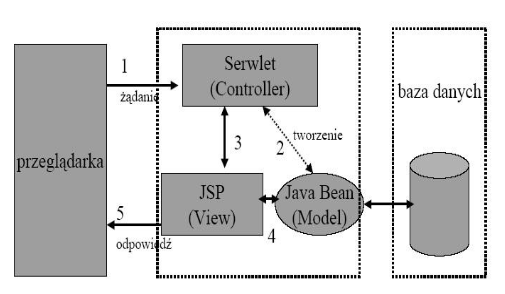
\includegraphics[width=12cm]{s4_int_jp100.png}
\caption{Współpraca JSP i serwletów - jako MVC (Model View Controller)}
\end{figure}

Następnym ważnym elementem występującym tym razem w warstwie biznesowej są \textbf{Enterprise Java Beans}. Jest to specyfikacja tworzenia aplikacji korporacyjnych. Opiera się ona na tworzeniu komponentów -- ziaren EJB, które są osadzane na serwerze aplikacji, a następnie ten serwer udostępnia je do wykonania lokalnie lub zdalnie (np. RMI). EJB tworzy rozproszoną, bezpieczną i transakcyjną klasę Java.

Ziarna EJB dzielą się na:
\begin{itemize}
    \item Session Beans -- stanowe (skojarzone z apl. klienta, pamiętają swój stan) oraz bezstanowe (może być za każdym razem używany przez innego klienta, pamięta tylko stan na czas wywołania)
    \item Message-Driven Beans
    \item Entity Beans (w EJB 3.0 zastąpione przez \textbf{JPA})
\end{itemize}

Każde z ziaren ma różne zastosowanie. Ziarna sesyjne są używane do umieszczania w nich logiki aplikacji -- czyli kodu, który przetwarza dane. Encyjne EJB reprezentują w sposób obiektowy dane (np. dostarczają obiektowego spojrzenia na relacyjną bazę danych). Ziarna sterowane komunikatami znajdują zastosowanie w przetwarzaniu asynchronicznym i w zaawansowanych modelach współpracy oprogramowania.

\textbf{RMI} -- Remote Method Invocation. Jest to protokół umożliwiający zdalne wywoływanie metod obiektów w aplikacjach Java. Obiekty te mogą znajdować się w innych maszynach wirtualnych Javy, które mogą znajdować się na innych komputerach. Obiekty zdalne rejestrowane są pod wybranymi nazwami w serwisie RMI Registry. Aplikacje korzystające z RMI dzielą prace na:
\begin{itemize}
    \item Odebranie żądania od klienta.
    \item Wykonanie zadania.
    \item Odesłanie odpowiedzi.
\end{itemize}

\textbf{JDBC} --  Java DataBase Connectivity. Odpowiednik ODBC dla Javy. Jest to interfejs oprogramowania pozwalający na połączenie z bazą danych SQL przez aplikacje Java.

\textbf{JPA} -- JavaPersistence API jest standardem ORM dla języka Java. Z punktu widzenia programisty jest to możliwość operowania na obiektach - zwanych encjami - oraz zapisywania wyników operacji do relacyjnej bazy danych za pomocą obiektu EntityManager. Implementacją która z tego korzysta jest np. \textbf{Hibernate}.

Popularne frameworki Java EE:

\textbf{Spring} -- Spring powstał jako alternatywa dla programowania aplikacji z użyciem Enterprise JavaBeans. Framework ma pomagać przy tworzeniu aplikacji na każdym poziomie. Ułatwia korzystanie z istniejących technologii.

\textbf{Play!} -- Inspirowany na Ruby on Rails oraz Django. Jest bezstanowy, RestFull. Bazuje na wzorcu MVC.

\textbf{Vaadin} -- używa Google Web Toolkit do generowania stron dla użyszkodnika. Wykorzystuje widgety oraz programowanie zdarzeniowe, więc tworzenie stron przypomina soft do tworzenia GUI, niż typowy webdev.